\documentclass[aspectratio=169]{beamer}

% ===================== THEME =====================
\usetheme{metropolis}
\setbeamertemplate{navigation symbols}{}
\setbeamertemplate{footline}[frame number]
\setbeamercovered{transparent}

\usepackage{comment}
\usepackage[utf8]{inputenc}
\usepackage{pifont}
\usepackage{tikz}
\usepackage{ifthen}
\usepackage{fontawesome5}
\usetikzlibrary{shapes.geometric, arrows.meta, positioning, fit, backgrounds, decorations.pathreplacing, calc}

\title[Deepfake Detection]{Deepfake Detection}
\subtitle{Seeing Is No Longer Believing}
\author{Md. Mufeed Talukder(151) \and Khandoker Md Tanjinul Islam(159) \and Md Tahmidul Islam(180)}
\institute{CSE 200}
\date{\today}

\begin{document}
% ===================================================
% SECTION: Introduction (Tahmid)
% Restyled to match Teammate 2's aesthetic:
%   - plain black-bordered boxes with light fills (no colored borders)
%   - footnotesize captions, \pause / <n-> reveals instead of decorative cards
%   - no frame transitions (\transfade etc. removed)
%   - photos shown plain, no outline boxes
% Order:
%   1. Title
%   2. Our Team (AI photo reveal)
%   3. The Threat and The Solution (icon-column definitions)
%   4. Audience Guessing Game (2 real / 2 fake images)
%   5. How Are They Generated? (creation flow)
%   6. Example: Source -> Target -> Outcome (single whole picture, no clicks)
%   7. Crisis of Trust (risks)
%   8. Handoff to Detection
% ===================================================

% ---------------------------------------------------
% SLIDE 1: Title Slide
% ---------------------------------------------------
\begin{frame}
\maketitle
\end{frame}

% ---------------------------------------------------
% SLIDE 2: Our Team (AI photo reveal -- plain, no boxes) [disabled]
% ---------------------------------------------------
% \begin{comment}
\begin{frame}{Our Team}
\centering
\begin{tikzpicture}
  \node[inner sep=0pt] (teamimg) {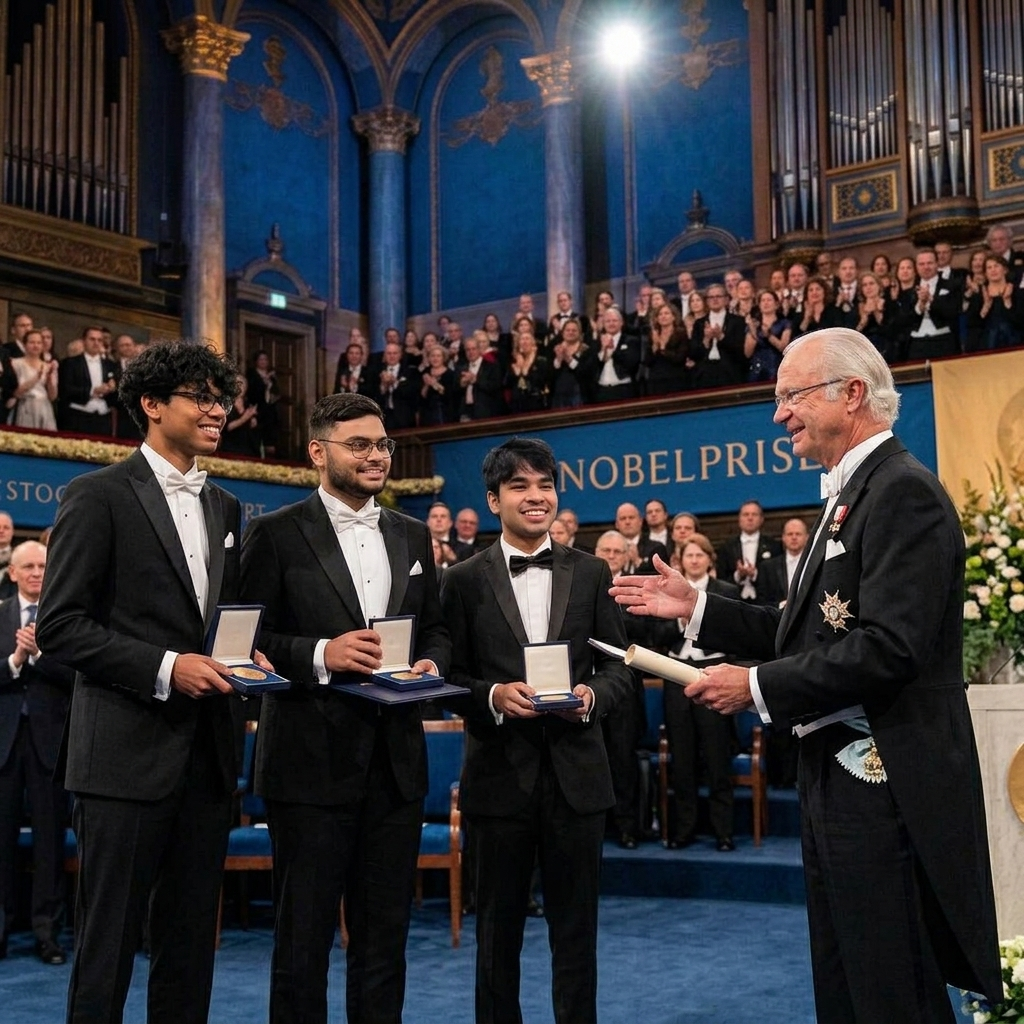
\includegraphics[width=8cm, height=4.5cm, keepaspectratio]{images/team_ai_photo}};
  \node[below=0.3cm of teamimg, align=center] {
    \textbf{Md. Mufeed Talukder} \hspace{0.5cm} \textbf{Khandoker Md Tanjinul Islam} \hspace{0.5cm} \textbf{Md Tahmidul Islam}
  };
\end{tikzpicture}

\vspace{0.4cm}
\pause
{\Large \textbf{Wait a second\ldots}}

\pause
\vspace{0.2cm}

{\Large \alert{We never Won the nobel prize}}
\end{frame}
% \end{comment}

% ---------------------------------------------------
% SLIDE 3: The Threat and The Solution (icon-column definitions)
% ---------------------------------------------------
\begin{frame}{The Threat and The Solution}
\centering
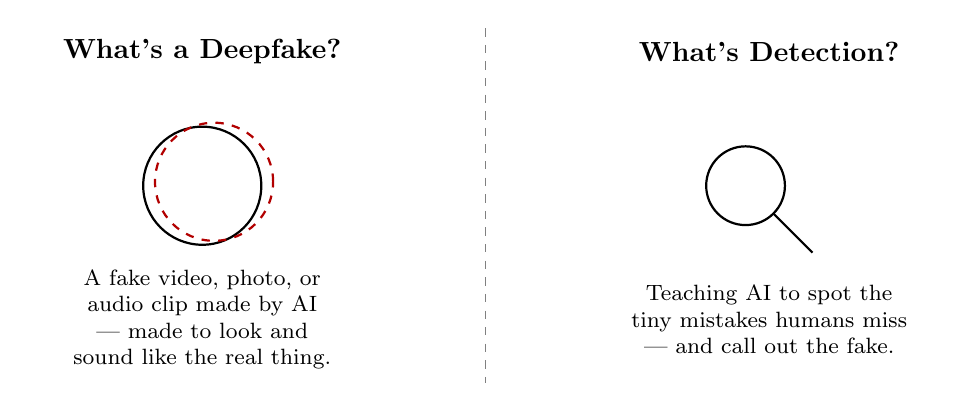
\begin{tikzpicture}[
  icon/.style={thick},
  lbl/.style={font=\bfseries},
  sub/.style={font=\footnotesize}
]
  % --- Deepfake (left) ---
  \node[lbl] (t1) at (-3.6,3.0) {What's a Deepfake?};
  \begin{scope}[shift={(-3.6,1.3)}]
    \draw[icon] (0,0) circle (0.75);
    \draw[icon, dashed, red!70!black] (0.15,0.05) circle (0.75);
  \end{scope}
  \node[sub, text width=4.2cm, align=center] at (-3.6,-0.4) {A fake video, photo, or audio clip made by AI --- made to look and sound like the real thing.};

  % --- divider ---
  \draw[dashed, gray] (0,3.3) -- (0,-1.2);

  % --- Detection (right) ---
  \onslide<2->{
  \node[lbl] (t2) at (3.6,3.0) {What's Detection?};
  \begin{scope}[shift={(3.6,1.3)}]
    \draw[icon] (-0.3,0) circle (0.5);
    \draw[icon] (0.05,-0.35) -- (0.55,-0.85);
  \end{scope}
  \node[sub, text width=4.2cm, align=center] at (3.6,-0.4) {Teaching AI to spot the tiny mistakes humans miss --- and call out the fake.};
  }
\end{tikzpicture}
\end{frame}

% ---------------------------------------------------
% SLIDE 4: Audience Guessing Game (2 Real / 2 Fake)
% ---------------------------------------------------
\begin{frame}{Can You Spot the Fake?}
\centering
{\Large \textbf{Real or Fake? Two of these are AI-generated.}}

\vspace{0.3cm}
\begin{tikzpicture}[imgcap/.style={font=\small}]
  \node<1->[inner sep=0pt] (img1) at (-3.3,1.3) {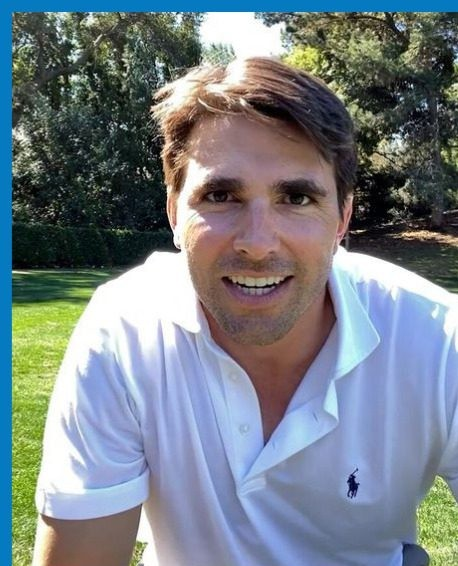
\includegraphics[width=4cm, height=2.4cm, keepaspectratio]{images/guess_1}};
  \node<1->[imgcap, below=0.1cm of img1] {Image 1};

  \node<1->[inner sep=0pt] (img2) at (3.3,1.3) {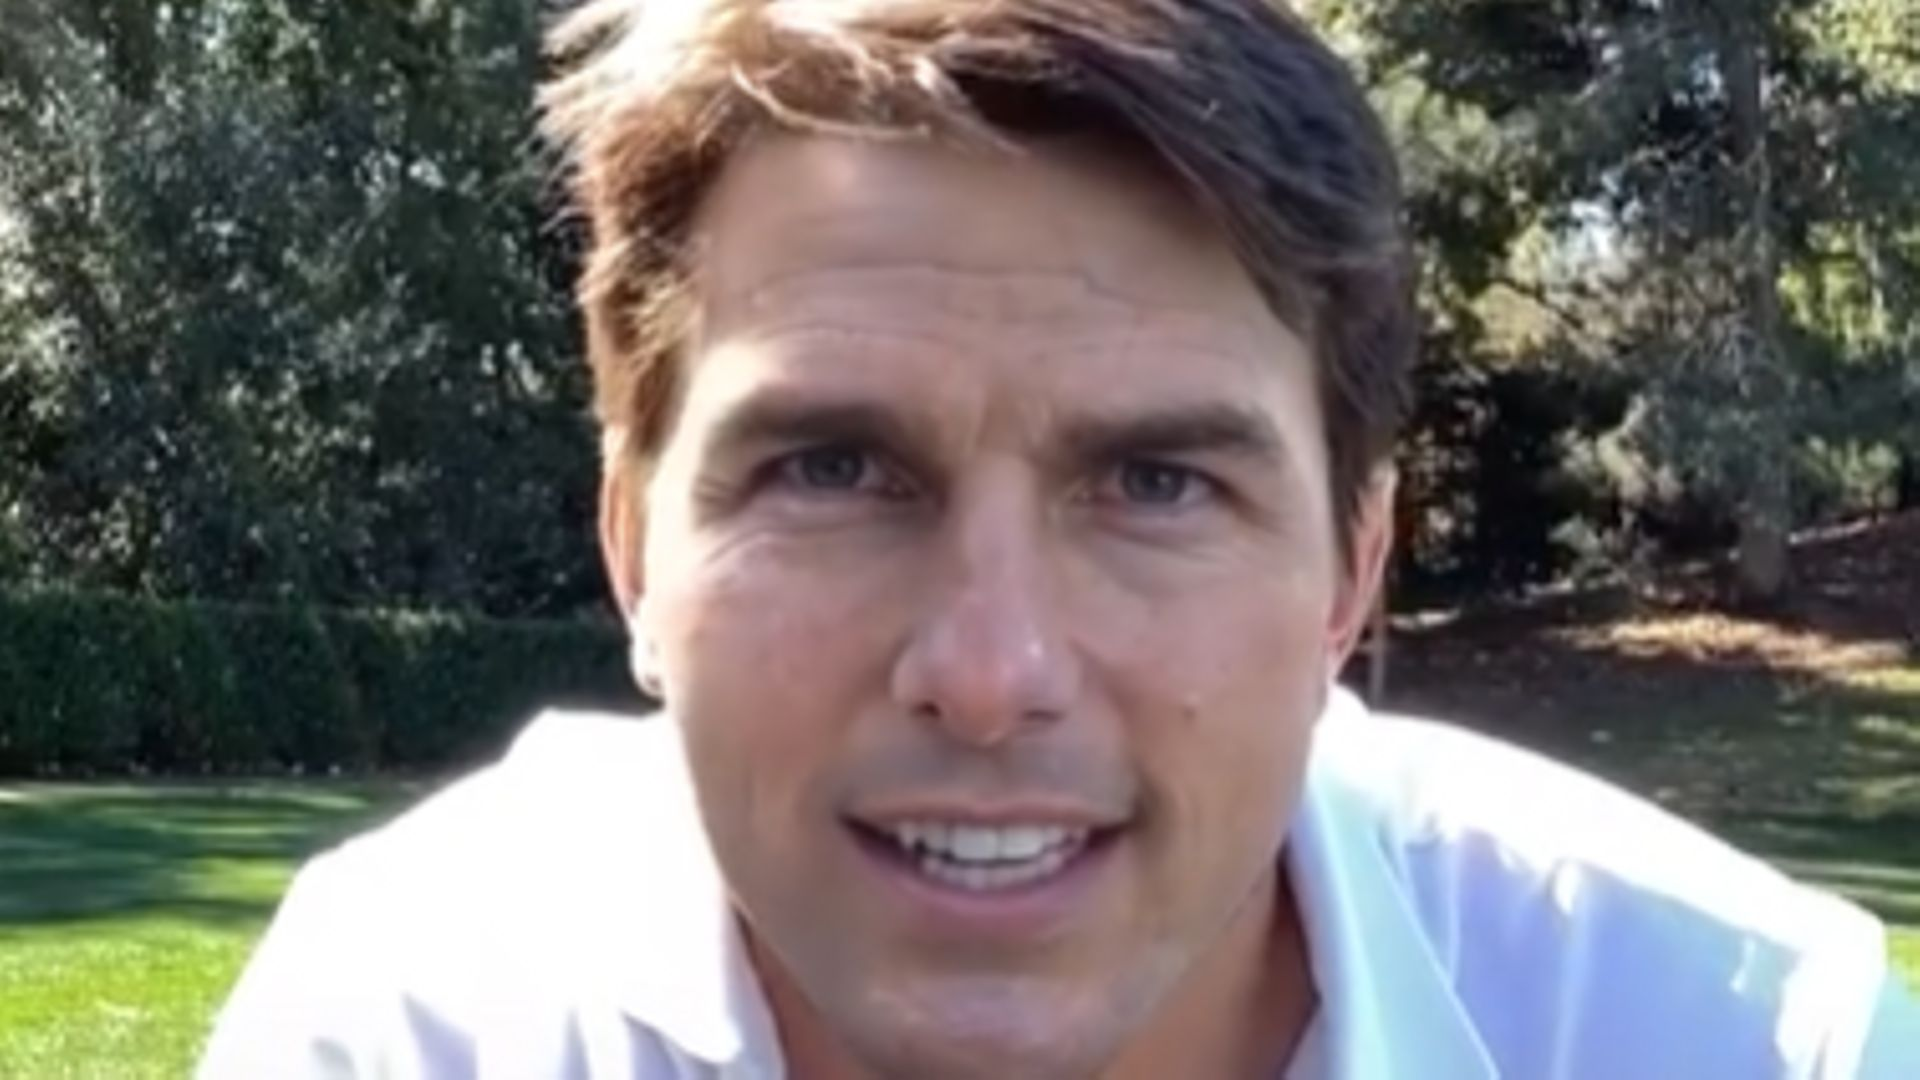
\includegraphics[width=4cm, height=2.4cm, keepaspectratio]{images/guess_2}};
  \node<1->[imgcap, below=0.1cm of img2] {Image 2};

  \node<1->[inner sep=0pt] (img3) at (-3.3,-1.9) {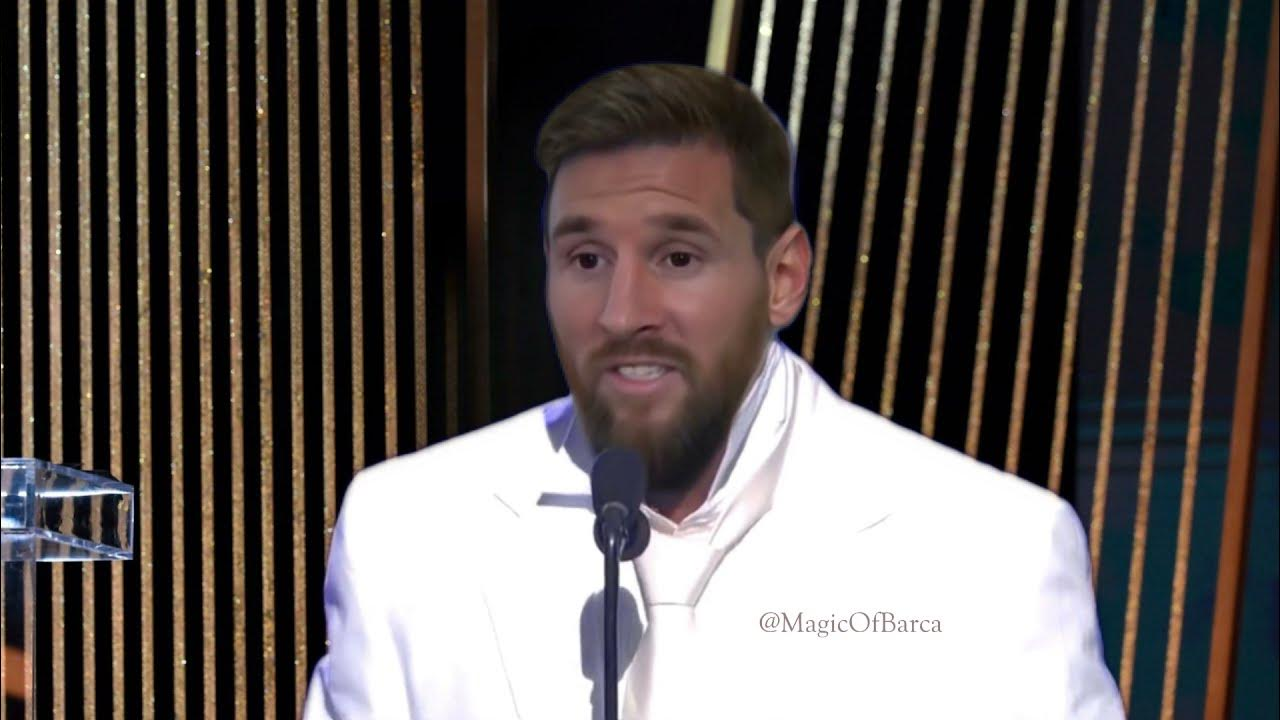
\includegraphics[width=4cm, height=2.4cm, keepaspectratio]{images/guess_3}};
  \node<1->[imgcap, below=0.1cm of img3] {Image 3};

  \node<1->[inner sep=0pt] (img4) at (3.3,-1.9) {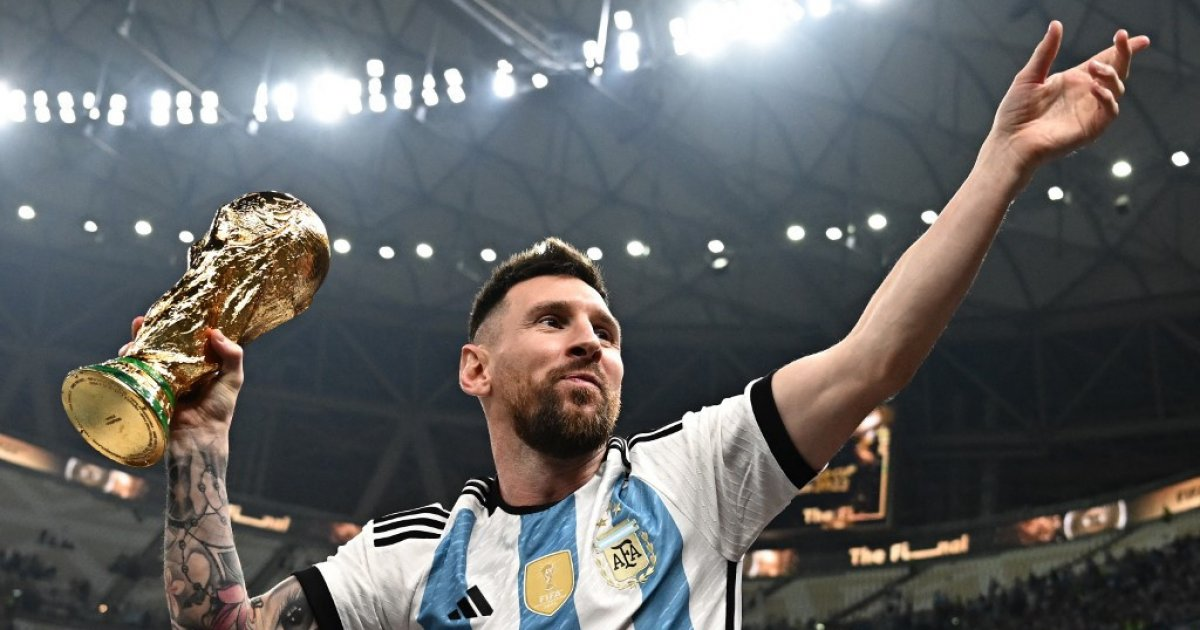
\includegraphics[width=4cm, height=2.4cm, keepaspectratio]{images/guess_4}};
  \node<1->[imgcap, below=0.1cm of img4] {Image 4};

  % Verdicts — plain thin boxes, light fill, black border (matches teammate 2's box style). Move to match your images.
  \node<2->[rectangle, rounded corners, draw, thick, fill=green!12, minimum width=1.4cm, minimum height=0.7cm, align=center] at (-1.9,2.55) {\footnotesize \textbf{REAL}};
  \node<2->[rectangle, rounded corners, draw, thick, fill=red!15, minimum width=1.4cm, minimum height=0.7cm, align=center] at (4.9,2.55) {\footnotesize \textbf{FAKE}};
  \node<2->[rectangle, rounded corners, draw, thick, fill=red!15, minimum width=1.4cm, minimum height=0.7cm, align=center] at (-1.9,-0.65) {\footnotesize \textbf{FAKE}};
  \node<2->[rectangle, rounded corners, draw, thick, fill=green!12, minimum width=1.4cm, minimum height=0.7cm, align=center] at (4.9,-0.65) {\footnotesize \textbf{REAL}};
\end{tikzpicture}

\pause
{\footnotesize \alert{If you hesitated even once --- that's the problem.}}
\end{frame}

% ---------------------------------------------------
% SLIDE 5: Generation Architecture (Any Media)
% ---------------------------------------------------
\begin{frame}{How Are They Generated?}
\centering
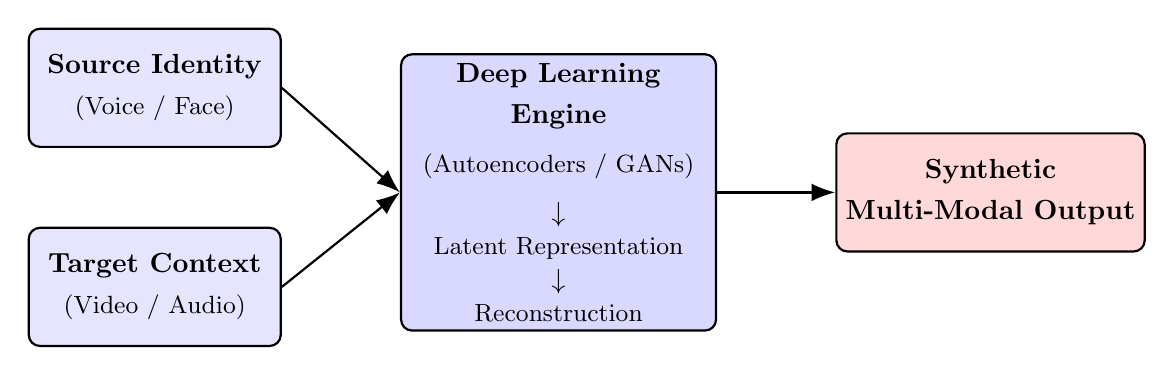
\begin{tikzpicture}[
  node distance=0.5cm,
  imgbox/.style={rectangle, rounded corners, draw, thick, fill=blue!10, minimum width=3.2cm, minimum height=1.5cm, align=center},
  net/.style={rectangle, rounded corners, draw, thick, fill=blue!15, minimum width=4cm, minimum height=3cm, align=center},
  arrowline/.style={-{Latex[length=3mm]}, thick}
]
  % Click 1: Source Identity
  \node<1->[imgbox] (facea) {\textbf{Source Identity}\\[0.1cm] \small (Voice / Face)};

  % Click 2: Target Context
  \node<2->[imgbox, below=1cm of facea] (faceb) {\textbf{Target Context}\\[0.1cm] \small (Video / Audio)};

  % Click 3: The Neural Network Engine
  \node<3->[net, right=1.5cm of faceb, yshift=1.2cm] (encdec) {
    \textbf{Deep Learning}\\[0.1cm]
    \textbf{Engine}\\[0.2cm]
    \small (Autoencoders / GANs)\\[0.2cm]
    $\downarrow$\\
    \small Latent Representation\\
    $\downarrow$\\
    \small Reconstruction
  };
  \draw<3->[arrowline] (facea.east) -- (encdec.west);
  \draw<3->[arrowline] (faceb.east) -- (encdec.west);

  % Click 4: The final fake output
  \node<4->[imgbox, right=1.5cm of encdec, fill=red!15] (fake) {\textbf{Synthetic}\\[0.1cm] \textbf{Multi-Modal Output}};
  \draw<4->[arrowline] (encdec.east) -- (fake.west);

\end{tikzpicture}
\end{frame}

% ---------------------------------------------------
% SLIDE 6: Example -- Source, Target, Outcome
% Shown as one whole picture (no clicks, no outline boxes around images)
% ---------------------------------------------------
\begin{frame}{Example: From Inputs to Output}
\centering
\begin{tikzpicture}[
  imgcap/.style={font=\small\bfseries},
  arrowline/.style={-{Latex[length=3mm]}, thick}
]
  \node[inner sep=0pt] (src) at (0,0) {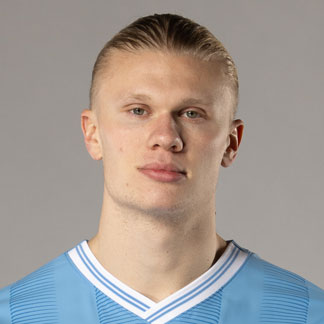
\includegraphics[width=3.2cm, height=2.2cm, keepaspectratio]{images/example_source}};
  \node[imgcap, below=0.15cm of src] {Source Image};

  \node[inner sep=0pt] (tgt) at (4.5,0) {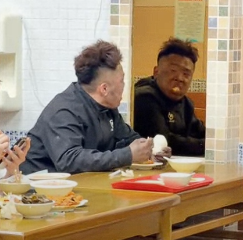
\includegraphics[width=3.2cm, height=2.2cm, keepaspectratio]{images/example_target}};
  \node[imgcap, below=0.15cm of tgt] {Target Image};

  \node[inner sep=0pt] (out) at (9,0) {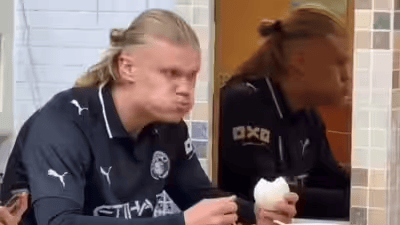
\includegraphics[width=3.2cm, height=2.2cm, keepaspectratio]{images/example_output}};
  \node[imgcap, below=0.15cm of out] {Outcome (Deepfake)};

  \draw[arrowline] (src.east) -- (tgt.west);
  \draw[arrowline] (tgt.east) -- (out.west);
\end{tikzpicture}
\end{frame}

% ---------------------------------------------------
% SLIDE 7: Crisis of Trust -- plain list, revealed one by one
% ---------------------------------------------------
\begin{frame}{The Crisis of Trust: A Weaponized Tool}
\centering
\begin{itemize}
  \item<1-> \textbf{Geopolitical Misinfo} --- fabricated speeches or events used to sway public opinion.
  \vspace{0.3cm}
  \item<2-> \textbf{Corporate Fraud} --- fake voices or video used to authorize scams and wire transfers.
  \vspace{0.3cm}
  \item<3-> \textbf{Identity Abuse} --- impersonation used for harassment or non-consensual content.
  \vspace{0.3cm}
  \item<4-> \textbf{Erosion of Evidence} --- makes real footage deniable, undermining trust in evidence itself.
\end{itemize}
\end{frame}

% ---------------------------------------------------
% SLIDE 8: The Handoff (Why We Need Detection)
% ---------------------------------------------------
\begin{frame}{Fighting Back}
\centering
\vspace{1cm}
{\Large \textbf{If Artificial Intelligence can forge reality,}}\\[0.3cm]
{\Large \textbf{can it also be trained to catch the forgery?}}

\vspace{0.8cm}
\pause
{\Huge $\Downarrow$}

\vspace{0.3cm}
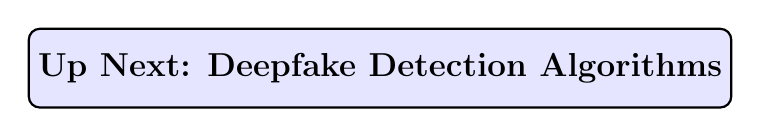
\begin{tikzpicture}
  \node[rectangle, rounded corners, draw, thick, fill=blue!10, minimum width=7cm, minimum height=1cm, align=center] {\large \textbf{Up Next: Deepfake Detection Algorithms}};
\end{tikzpicture}
\end{frame}
% ===================================================
% SECTION: Detection Techniques (Teammate 2)
% ===================================================
\section{Detection Techniques}

% ---------------------------------------------------
% SLIDE 1: The Two Fronts of Detection
% ---------------------------------------------------
\begin{frame}{The Two Fronts of Detection}
\centering
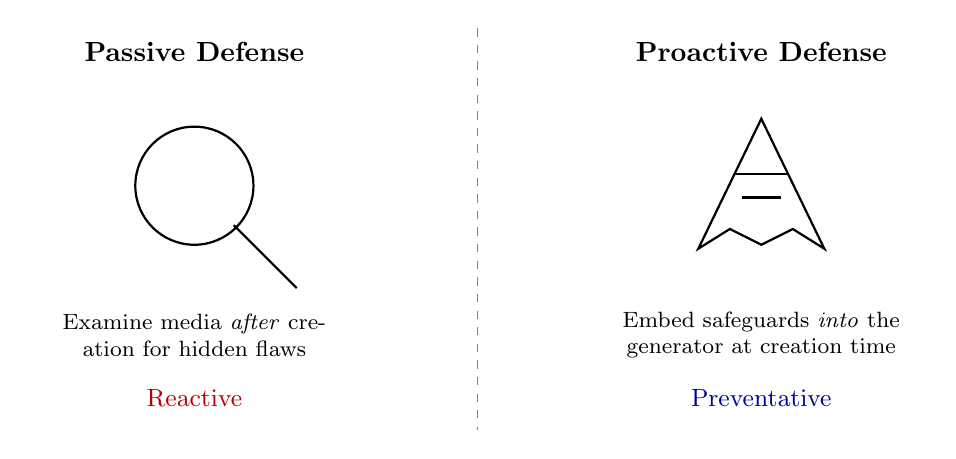
\begin{tikzpicture}[
  icon/.style={thick},
  lbl/.style={font=\bfseries},
  sub/.style={font=\footnotesize}
]
  % --- Passive Defense (left) ---
  \node[lbl] (t1) at (-3.6,3.0) {Passive Defense};
  \begin{scope}[shift={(-3.6,1.3)}]
    \draw[icon] (0,0) circle (0.75);
    \draw[icon] (0.5,-0.5) -- (1.3,-1.3);
  \end{scope}
  \node[sub, text width=4cm, align=center] at (-3.6,-0.6) {Examine media \emph{after} creation for hidden flaws};
  \node[font=\small, red!70!black] at (-3.6,-1.4) {Reactive};

  % --- divider ---
  \draw[dashed, gray] (0,3.3) -- (0,-1.8);

  % --- Proactive Defense (right) ---
  \onslide<2->{
  \node[lbl] (t2) at (3.6,3.0) {Proactive Defense};
  \begin{scope}[shift={(3.6,1.3)}]
    \draw[icon] (-0.8,-0.8) -- (0,0.85) -- (0.8,-0.8) -- (0.4,-0.55) -- (0,-0.75) -- (-0.4,-0.55) -- cycle;
    \draw[icon] (-0.35,0.15) -- (0.35,0.15);
    \draw[icon] (-0.25,-0.15) -- (0.25,-0.15);
  \end{scope}
  \node[sub, text width=4cm, align=center] at (3.6,-0.6) {Embed safeguards \emph{into} the generator at creation time};
  \node[font=\small, blue!60!black] at (3.6,-1.4) {Preventative};
  }
\end{tikzpicture}

\vspace{0.2cm}
\pause
{\footnotesize \alert{It's a cat-and-mouse game} --- every new detector eventually meets a generator built to beat it.}
\end{frame}

% ---------------------------------------------------
% SLIDE 2: Passive Detection -- Spatial Artifacts
% ---------------------------------------------------
\begin{frame}{Passive Detection: Spatial Artifacts}
\centering
\begin{columns}[c]
  \column{0.48\textwidth}
  \centering
  \begin{tikzpicture}
    \node[inner sep=0pt] (photo) at (0,0) {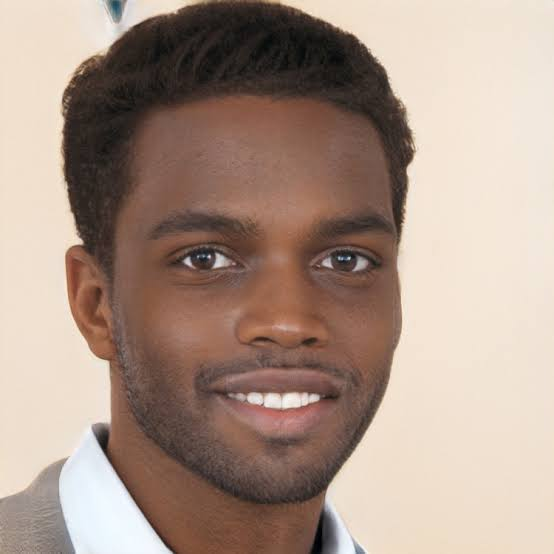
\includegraphics[width=3.4cm]{images/face_photo.png}};
    % unnaturally smooth / waxy forehead
    \draw[very thick, dashed, red] (0.05,0.9) ellipse (0.55 and 0.45);
    \node[red, font=\footnotesize, align=center] at (-2.05,1.3) {unnaturally\\smooth forehead};
    \draw[->, red, thick] (-1.15,1.15) -- (-0.4,1.0);
    % even focus -- face and background equally sharp
    \draw[very thick, dashed, teal] (1.3,0.55) ellipse (0.3 and 0.45);
    \node[teal!70!black, font=\footnotesize, align=center] at (2.55,0.1) {no depth blur:\\even focus};
    \draw[->, teal!70!black, thick] (2.0,0.3) -- (1.6,0.5);
  \end{tikzpicture}

  \column{0.48\textwidth}
  \centering
  \begin{tikzpicture}[
    node distance=0.7cm,
    net/.style={rectangle, rounded corners, draw, thick, minimum width=2.6cm, minimum height=1.2cm, fill=blue!15, align=center},
    outbox/.style={rectangle, rounded corners, draw, thick, minimum width=2.6cm, minimum height=1cm, fill=gray!10, align=center},
    arrowline/.style={-{Latex[length=3mm]}, thick}
  ]
    \onslide<3->{\node[draw, thick, inner sep=1pt] (frame) {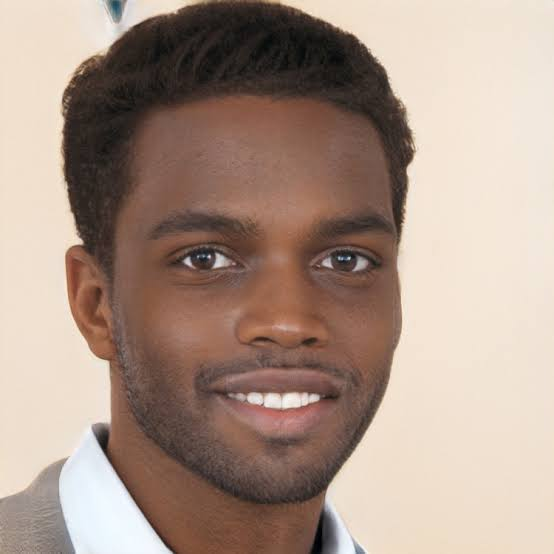
\includegraphics[width=2.1cm]{images/face_photo.png}};}
    \onslide<3->{
    \node[net, below=of frame] (cnn) {CNN};
    \node[outbox, below=of cnn, fill=orange!15] (out) {Real / Fake};
    \draw[arrowline] (frame) -- (cnn);
    \draw[arrowline] (cnn) -- (out);
    }
  \end{tikzpicture}
\end{columns}

\vspace{0.15cm}
\onslide<3->{\footnotesize A single frame is enough: waxy, over-smoothed skin and an unnatural lack of depth-of-field are learned by a standard CNN.}

\only<2>{
\begin{tikzpicture}[remember picture, overlay]
  \node[rotate=12, draw=red!70!black, ultra thick, rounded corners, fill=red!8,
        inner sep=10pt, font=\fontsize{34}{40}\selectfont\bfseries,
        text=red!70!black] at ($(current page.center)+(0,0.3)$) {\textbf{!!}\; RED FLAGS \;\textbf{!!}};
\end{tikzpicture}
}
\end{frame}

% ---------------------------------------------------
% SLIDE 3: Passive Detection -- Temporal Artifacts
% ---------------------------------------------------
\begin{frame}{Passive Detection: Temporal Artifacts}
\centering
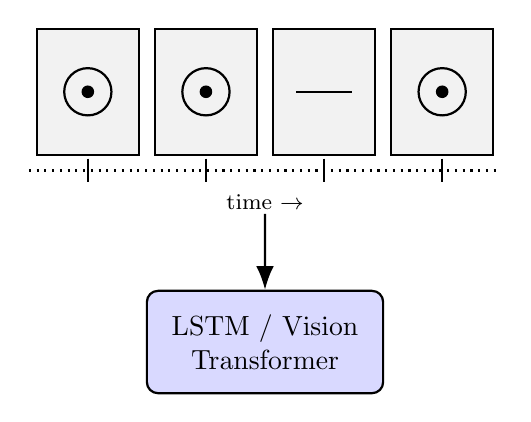
\begin{tikzpicture}[
  frm/.style={rectangle, draw, thick, minimum width=1.3cm, minimum height=1.6cm, fill=gray!10},
  net/.style={rectangle, rounded corners, draw, thick, minimum width=3cm, minimum height=1.3cm, fill=blue!15, align=center},
  arrowline/.style={-{Latex[length=3mm]}, thick}
]
  % filmstrip of 4 frames with an eye that blinks
  \foreach \i/\x/\eye in {1/0/open, 2/1.5/open, 3/3.0/closed, 4/4.5/open} {
    \node[frm] (f\i) at (\x,0) {};
    \ifthenelse{\equal{\eye}{closed}}
      {\draw[thick] (\x-0.35,0) -- (\x+0.35,0);}
      {\draw[thick] (\x,0) circle (0.3); \fill (\x,0) circle (0.08);}
  }
  \draw[dotted, thick] (-0.75,-1.0) -- (5.25,-1.0);
  \foreach \x in {0,1.5,3.0,4.5} { \draw[thick] (\x,-0.85) -- (\x,-1.15); }
  \node[font=\footnotesize] at (2.25,-1.4) {time $\rightarrow$};

  \onslide<2->{
  \node[net, below=1.7cm of f1, xshift=2.25cm] (rnn) {LSTM / Vision\\Transformer};
  \draw[arrowline] (2.25,-1.55) -- (rnn);
  }
\end{tikzpicture}

\vspace{0.2cm}
\pause
{\footnotesize Fakes struggle to stay consistent \emph{across} frames: unnatural blink rates, jerky motion, missing heartbeat-driven skin-color shifts.}
\end{frame}

% ---------------------------------------------------
% SLIDE 4: The Multimodal Frontier (Audio + Video)
% ---------------------------------------------------
\begin{frame}{The Multimodal Frontier: Audio Meets Video}
\centering
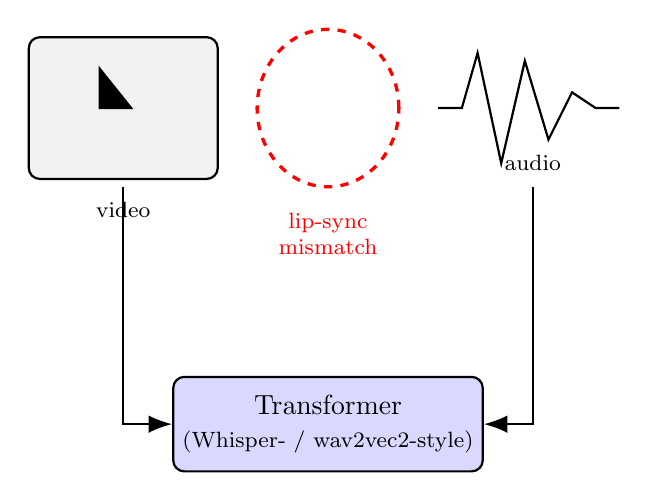
\begin{tikzpicture}[
  net/.style={rectangle, rounded corners, draw, thick, minimum width=3.4cm, minimum height=1.2cm, fill=blue!15, align=center},
  arrowline/.style={-{Latex[length=3mm]}, thick}
]
  % video play icon
  \node[draw, thick, rounded corners, minimum width=2.4cm, minimum height=1.8cm, fill=gray!10] (vid) at (-2.6,1.0) {};
  \draw[thick, fill=black] (-2.9,1.0) -- (-2.9,1.5) -- (-2.5,1.0) -- cycle;
  \node[below=0.15cm of vid, font=\footnotesize] {video};

  % waveform icon
  \node (wav) at (2.6,1.0) {};
  \draw[thick] (1.4,1.0) -- (1.7,1.0) -- (1.9,1.7) -- (2.2,0.3) -- (2.5,1.6) -- (2.8,0.6) -- (3.1,1.2) -- (3.4,1.0) -- (3.7,1.0);
  \node[below=0.35cm of wav, font=\footnotesize] {audio};

  \draw[very thick, dashed, red] (0,1.0) ellipse (0.9 and 1.0);
  \node[red, font=\footnotesize, align=center] at (0,-0.6) {lip-sync\\mismatch};

  \onslide<2->{
  \node[net, below=1.4cm of {(0,-1.0)}] (trf) {Transformer\\\footnotesize(Whisper- / wav2vec2-style)};
  \draw[arrowline] (-2.6,0.0) |- (trf.west);
  \draw[arrowline] (2.6,0.0) |- (trf.east);
  }
\end{tikzpicture}

\vspace{0.15cm}
\pause
{\footnotesize Voice can be faked too. Cross-checking acoustic cues against mouth movement --- e.g.\ does a ``B'' sound match a closed mouth? --- exposes synthetic audio.}
\end{frame}

% ---------------------------------------------------
% SLIDE 5: Proactive Defense -- AI Watermarking
% ---------------------------------------------------

\begin{frame}{Proactive Defense: Invisible Watermarking}
\centering
\resizebox{\textwidth}{!}{%
\begin{tikzpicture}[
  every node/.style={font=\small},
  nn/.style={circle, draw, fill=gray!10, minimum size=4mm, inner sep=0pt}
]

% ---------- AI GENERATIVE MODEL BOX ----------
\node[draw, rounded corners, fill=gray!5, minimum width=3.8cm, minimum height=3.2cm]
  (genbox) at (-5.0,0) {};
\node[font=\bfseries\small, align=center] at (-5.0,1.95) {AI Generative Model};

% inputs
\node[align=right, font=\footnotesize] (prompt) at (-8.2,0.55) {Text\\Prompt};
\node[align=right, font=\footnotesize] (context) at (-8.2,-0.55) {Context\\Data};
\draw[-{Latex[length=2.5mm]}] (prompt.east) -- (-6.85,0.55);
\draw[-{Latex[length=2.5mm]}] (context.east) -- (-6.85,-0.55);

% mini neural network, layered
\foreach \y [count=\i] in {0.7,0.25,-0.25,-0.7}
  \node[nn] (in\i) at (-6.5,\y) {};
\foreach \y [count=\i] in {0.75,0.35,-0.05,-0.45,-0.85}
  \node[nn] (hid\i) at (-5.95,\y) {};
\foreach \y [count=\i] in {0.35,-0.35}
  \node[nn] (out\i) at (-5.4,\y) {};

\foreach \i in {1,...,4}
  \foreach \j in {1,...,5}
    \draw[gray!60, thin] (in\i) -- (hid\j);
\foreach \j in {1,...,5}
  \foreach \k in {1,...,2}
    \draw[gray!60, thin] (hid\j) -- (out\k);

% key + watermark embedder
% \node[font=\large] (key) at (-4.6,1.15) {\faKey};
% \node[font=\tiny, align=center] at (-4.6,1.5) {Cryptographic Key};
% \draw[-{Latex[length=2mm]}, thin] (key) -- (-4.6,0.5);

% \node[draw, rounded corners, fill=gray!15, minimum width=1.9cm, minimum height=0.9cm,
%       align=center, font=\tiny, inner sep=3pt] (embedder) at (-4.6,0.0) {Watermark\\Embedder};
\begin{scope}[shift={(0.4cm,-0.65cm)}]

\node[font=\large] (key) at (-4.6,1.15) {\faKey};
\node[font=\tiny, align=center] at (-4.6,1.5) {Cryptographic Key};
\draw[-{Latex[length=2mm]}, thin] (key) -- (-4.6,0.5);

\node[draw, rounded corners, fill=gray!15, minimum width=1.9cm, minimum height=0.9cm,
      align=center, font=\tiny, inner sep=3pt] (embedder) at (-4.6,0.0)
      {Watermark\\Embedder};

\end{scope}
% ---------- FACE IMAGE ----------
\node[inner sep=0pt] (face) at (0,0)
  {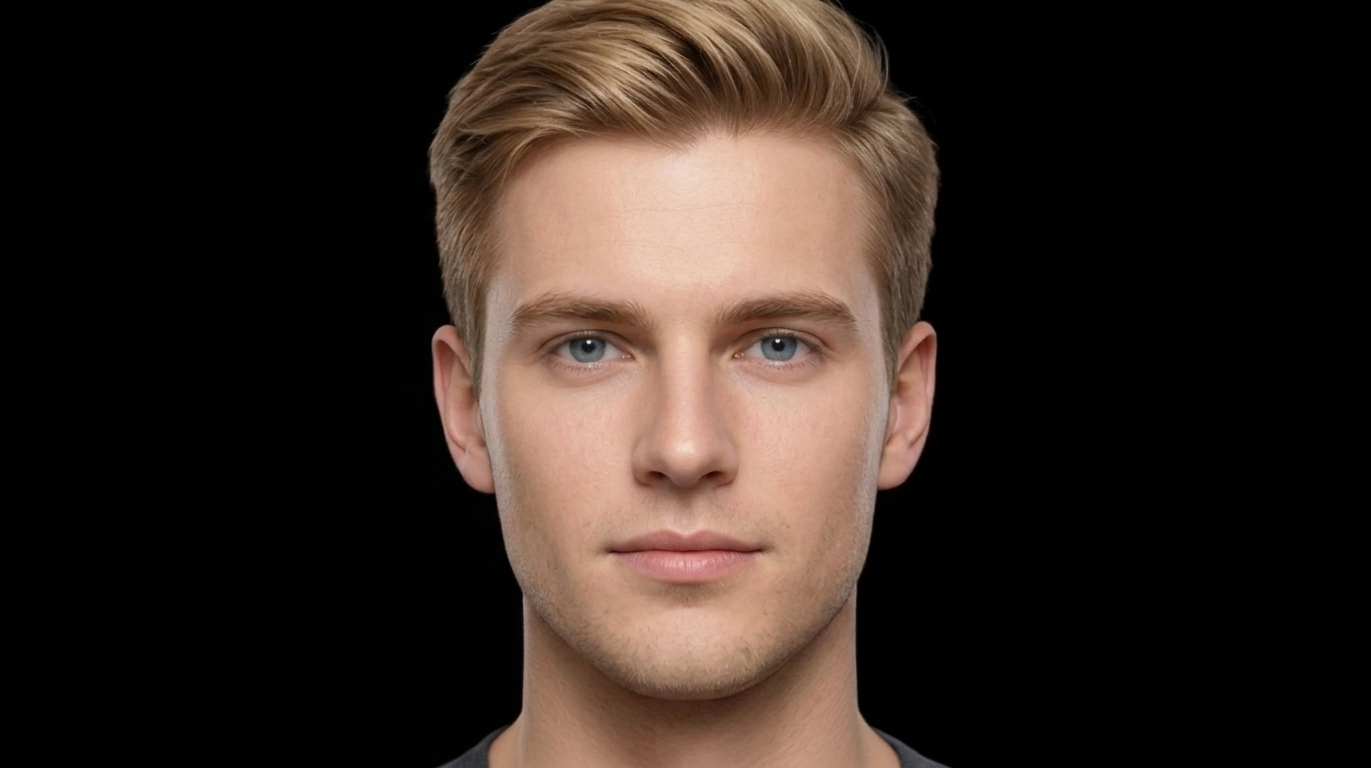
\includegraphics[width=2.4cm]{images/syn.jpg}};

\draw[-{Latex[length=3mm]}, thick] (-3.1,0) -- (-1.35,0);

% magnifying glass over bottom-right corner of face
\node[font=\large] at (0.95,-1.0) {\faSearch};

% zoomed pattern inset -- pulled down and left, away from verification caption
\node[draw, thick, fill=green!8, minimum width=1.9cm, minimum height=0.9cm]
  (zoom) at (2.15,-2.1) {};
\node[font=\tiny\ttfamily, green!40!black, align=left] at (2.15,-2.1)
  {01011001\\10110010\\01101011};
\draw[thin] (1.15,-0.7) -- (1.6,-1.75);
\draw[thin] (1.3,-1.25) -- (2.4,-1.65);

\node[font=\tiny, blue!50!black, align=center] at (-4.6,-2.0)
  {imperceptible cryptographic pattern\\embedded at generation time};
\node[font=\small, align=center] at (-0.8,-2.0)
  {Perceptually Clean\\AI-Generated Media};

% ---------- VERIFICATION SYSTEM ----------
\draw[-{Latex[length=3mm]}, thick] (1.35,0) -- (3.1,0);

\node[draw, rounded corners, fill=gray!5, minimum width=2.5cm, minimum height=1.6cm]
  (verifbox) at (4.4,0) {};
\node[font=\bfseries\tiny, align=center] at (4.4,0.95) {Verification System};
\node[font=\large] at (4.05,0.15) {\faMicroscope};
\node[font=\large] at (4.75,0.15) {\faCode};
\node[font=\tiny, align=center] at (4.4,-0.5) {Extracts and checks\\for pattern match};

% ---------- VERIFIED ----------
\draw[-{Latex[length=3mm]}, thick] (5.65,0) -- (6.75,0);
\node[rectangle, rounded corners, draw, thick, fill=green!12,
      minimum width=2.5cm, minimum height=1cm, align=center] (verify) at (8.1,0)
  {\small Verified:\\\footnotesize AI-Generated};

\end{tikzpicture}%
}

\vspace{0.2cm}
{\footnotesize Survives compression, cropping, and screenshots --- so platforms can confirm origin without any loss in quality.}
\end{frame}
% ---------------------------------------------------
% SLIDE 6: Summary & The Road Ahead
% ---------------------------------------------------
\begin{frame}{Summary: No Silver Bullet}
\centering
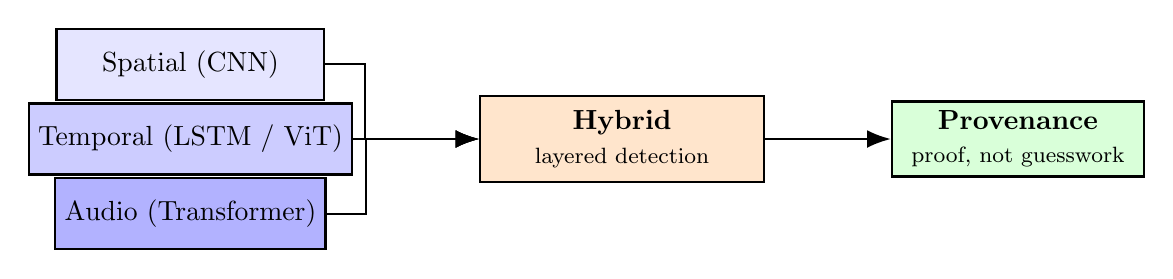
\begin{tikzpicture}[
  layer/.style={rectangle, draw, thick, minimum width=3.4cm, minimum height=0.9cm, align=center},
  arrowline/.style={-{Latex[length=3mm]}, thick}
]
  \node[layer, fill=blue!10] (l1) at (0,2.0) {Spatial (CNN)};
  \node[layer, fill=blue!20] (l2) at (0,1.05) {Temporal (LSTM / ViT)};
  \node[layer, fill=blue!30] (l3) at (0,0.1) {Audio (Transformer)};

  \onslide<2->{
  \node[layer, fill=orange!20, minimum width=3.6cm, minimum height=1.1cm, right=1.6cm of l2] (hyb) {\textbf{Hybrid}\\\footnotesize layered detection};
  \draw[arrowline] (l1.east) -- ++(0.5,0) |- (hyb.west);
  \draw[arrowline] (l2.east) -- (hyb.west);
  \draw[arrowline] (l3.east) -- ++(0.5,0) |- (hyb.west);
  }

  \onslide<3->{
  \node[layer, fill=green!15, minimum width=3.2cm, right=1.6cm of hyb] (prov) {\textbf{Provenance}\\\footnotesize proof, not guesswork};
  \draw[arrowline] (hyb) -- (prov);
  }
\end{tikzpicture}

\vspace{0.2cm}
\pause\pause\pause
{\footnotesize The field is shifting from playing detective --- hunting for AI mistakes --- to demanding cryptographic proof of authenticity.}
\end{frame}

% ===================================================
% BRIDGE: Detection -> Applications
% ===================================================
\begin{frame}{Detection Works in the Lab --- But Does It Survive Real Life?}
\centering
\vspace{1cm}
{\Large \textbf{We can now spot a fake in a single frame.}}\\[0.3cm]
{\Large \textbf{But can our tools survive the internet, the courtroom, the real world?}}

\vspace{0.8cm}
\pause
{\Huge $\Downarrow$}

\vspace{0.3cm}
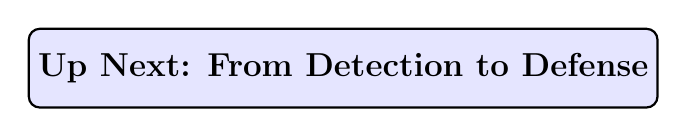
\begin{tikzpicture}
  \node[rectangle, rounded corners, draw, thick, fill=blue!10, minimum width=7cm, minimum height=1cm, align=center] {\large \textbf{Up Next: From Detection to Defense}};
\end{tikzpicture}
\end{frame}

% ===================================================
% SECTION: Applications & Outlook (Teammate 3)
% ===================================================
\section{From Detection to Defense}

% ---------------------------------------------------
% SLIDE 1: Where Detection Matters
% Speaking cue: give ONE concrete example per icon out loud
% (e.g. "TikTok scanning uploads", "a bank verifying a face
% for a loan", "a journalist checking a leaked clip").
% ---------------------------------------------------
\begin{frame}{Where Detection Matters}
\centering
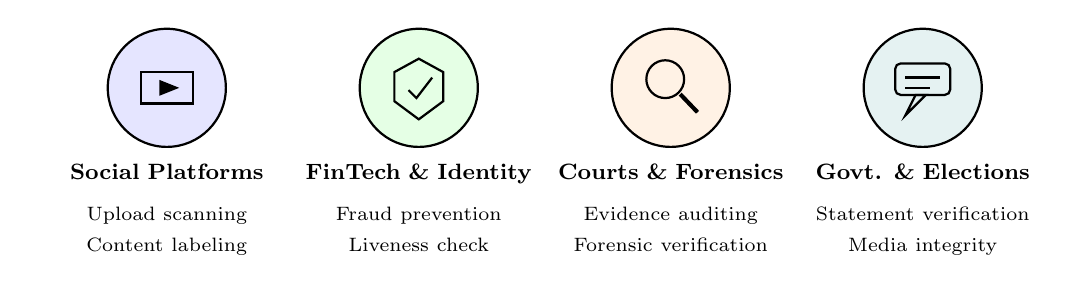
\begin{tikzpicture}[capt/.style={font=\footnotesize, align=center, text width=3.3cm}]

  % --- Social Platforms ---
  \begin{scope}[shift={(-4.8,0)}]
    \draw[thick, fill=blue!10] (0,0) circle (0.75);
    \draw[thick] (-0.33,-0.2) rectangle (0.33,0.2);
    \draw[thick, fill=black] (-0.08,-0.08) -- (-0.08,0.08) -- (0.12,0) -- cycle;
    \node[capt, below=0.85cm] {
      \textbf{Social Platforms}\\[0.18cm]
      {\scriptsize Upload scanning}\\[0.06cm]
      {\scriptsize Content labeling}
    };
  \end{scope}

  % --- FinTech & Identity ---
  \onslide<2->{
  \begin{scope}[shift={(-1.6,0)}]
    \draw[thick, fill=green!10] (0,0) circle (0.75);
    \draw[thick] (0,0.37) -- (0.31,0.2) -- (0.31,-0.17) -- (0,-0.4) -- (-0.31,-0.17) -- (-0.31,0.2) -- cycle;
    \draw[thick] (-0.13,-0.03) -- (-0.03,-0.13) -- (0.17,0.13);
    \node[capt, below=0.85cm] {
      \textbf{FinTech \& Identity}\\[0.18cm]
      {\scriptsize Fraud prevention}\\[0.06cm]
      {\scriptsize Liveness check}
    };
  \end{scope}
  }

  % --- Courts & Forensics ---
  \onslide<3->{
  \begin{scope}[shift={(1.6,0)}]
    \draw[thick, fill=orange!10] (0,0) circle (0.75);
    \draw[thick] (-0.07,0.11) circle (0.24);
    \draw[thick, line width=1.5pt] (0.12,-0.08) -- (0.34,-0.31);
    \node[capt, below=0.85cm] {
      \textbf{Courts \& Forensics}\\[0.18cm]
      {\scriptsize Evidence auditing}\\[0.06cm]
      {\scriptsize Forensic verification}
    };
  \end{scope}
  }

  % --- Journalism & Elections ---
  \onslide<4->{
  \begin{scope}[shift={(4.8,0)}]
    \draw[thick, fill=teal!10] (0,0) circle (0.75);
    \draw[thick, rounded corners=2pt] (-0.35,-0.09) rectangle (0.35,0.31);
    \draw[thick] (-0.09,-0.09) -- (-0.22,-0.35) -- (0.04,-0.09) -- cycle;
    \draw[thick] (-0.22,0.13) -- (0.22,0.13);
    \draw[thick] (-0.22,0.0) -- (0.09,0.0);
    \node[capt, below=0.85cm] {
      \textbf{Govt. \& Elections}\\[0.18cm]
      {\scriptsize Statement verification}\\[0.06cm]
      {\scriptsize Media integrity}
    };
  \end{scope}
  }

\end{tikzpicture}

\vspace{0.8cm}
\onslide<5->{{\footnotesize Different environments \alert{\textit{demand}} different guarantees.}}
\end{frame}

% ---------------------------------------------------
% SLIDE 2: Defense in Depth
% Speaking cue: walk left to right -- prevention, detection,
% verification are three separate layers, not one silver bullet.
% ---------------------------------------------------
\begin{frame}{The Future Is Not ``One Detector''}
\centering
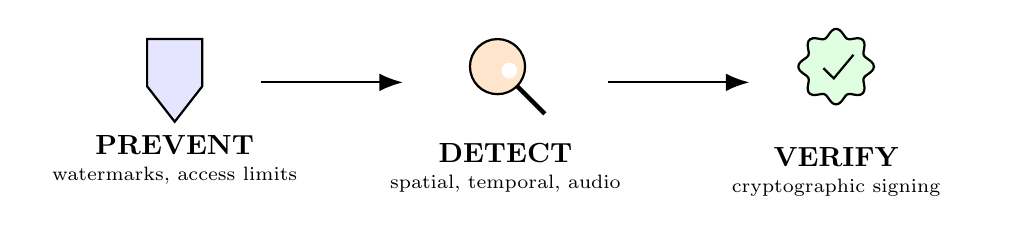
\begin{tikzpicture}[
  lbl/.style={font=\bfseries},
  ex/.style={font=\scriptsize, align=center, text width=3.5cm},
  arrowline/.style={-{Latex[length=3mm]}, thick}
]
  % PREVENT
  \begin{scope}[shift={(-4.2,0.3)}]
    \draw[thick, fill=blue!10] (-0.35,0.55) -- (0.35,0.55) -- (0.35,-0.05) -- (0,-0.5) -- (-0.35,-0.05) -- cycle;
    \node[lbl, below=0.55cm] (l1) {PREVENT};
    \node[ex, below=0.95cm] {watermarks, access limits};
  \end{scope}

  \draw[arrowline] (-3.1,0.3) -- (-1.3,0.3);

  % DETECT
  \begin{scope}[shift={(0,0.3)}]
    \draw[thick, fill=orange!20] (-0.1,0.2) circle (0.35);
    \draw[draw=none, fill=white] (0.05,0.15) circle (0.1);
    \draw[thick, line width=1.6pt] (0.15,-0.05) -- (0.5,-0.4);
    \node[lbl, below=0.65cm] {DETECT};
    \node[ex, below=1.05cm] {spatial, temporal, audio};
  \end{scope}

  \draw[arrowline] (1.3,0.3) -- (3.1,0.3);

% VERIFY
  \begin{scope}[shift={(4.2,0.3)}]
    % Wavy outer seal / rosette border
    \draw[thick, fill=green!12, domain=0:360, samples=90, smooth cycle]
      plot ({0 + (0.43 + 0.05*cos(8*\x))*cos(\x)}, {0.2 + (0.43 + 0.05*cos(8*\x))*sin(\x)});
    % Checkmark
    \draw[thick] (-0.16,0.18) -- (-0.03,0.05) -- (0.22,0.35);
    \node[lbl, below=0.7cm] {VERIFY};
    \node[ex, below=1.1cm] {cryptographic signing};
  \end{scope}

\end{tikzpicture}

\vspace{1.6cm}
\pause
{\large \textbf{Defense in depth beats a single ``AI detector.''}}
\end{frame}

% ---------------------------------------------------
% SLIDE 3: The Future of Authenticity
% Speaking cue: "good news" beat -- detection alone can't win
% the arms race, so the industry proves origin instead.
% ---------------------------------------------------
\begin{frame}{The Future of Authenticity: Proving Where Content Came From}
\centering
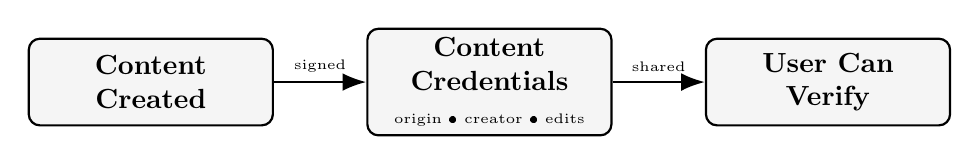
\begin{tikzpicture}[
  box/.style={rectangle, rounded corners, draw, thick, minimum width=3.1cm, minimum height=1.1cm, align=center, fill=gray!8},
  arrowline/.style={-{Latex[length=3mm]}, thick},
  alabel/.style={font=\tiny, align=center}
]
  \node[box] (created) at (-4.3,0) {\textbf{Content}\\\textbf{Created}};
  \node[box] (cred) at (0,0) {\textbf{Content}\\\textbf{Credentials}\\{\tiny origin \textbullet\ creator \textbullet\ edits}};
  \node[box] (verify) at (4.3,0) {\textbf{User Can}\\\textbf{Verify}};

  \draw[arrowline] (created) -- node[alabel, above] {signed} (cred);
  \draw[arrowline] (cred) -- node[alabel, above] {shared} (verify);
\end{tikzpicture}

\vspace{0.9cm}
\onslide<2->{
{\footnotesize \textbf{Detection asks:} \textit{``Does this look fake?''}}\\[0.15cm]
{\footnotesize \textbf{Provenance asks:} \textit{``Can we prove where it came from?''}}
}

\vspace{0.5cm}
\pause
{\tiny C2PA / Content Credentials --- an emerging industry standard.}
\end{frame}

% ---------------------------------------------------
% SLIDE 4: The Road Ahead (predictions + closing loop-back)
% ---------------------------------------------------
\begin{frame}{The Road Ahead}
\centering
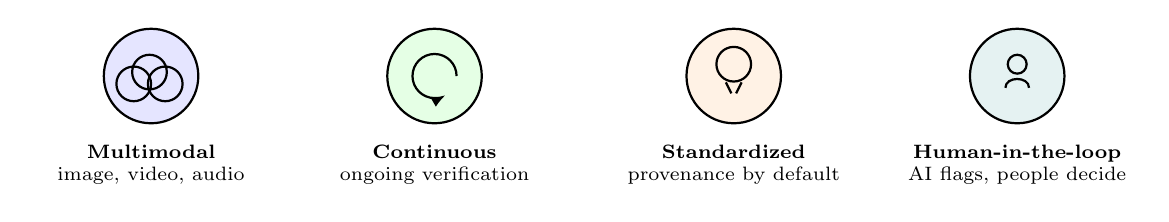
\begin{tikzpicture}[capt/.style={font=\scriptsize, align=center, text width=2.9cm}]

  \begin{scope}[shift={(-5.5,0)}]
    \draw[thick, fill=blue!10] (0,0) circle (0.6);
    \draw[thick] (-0.22,-0.1) circle (0.22);
    \draw[thick] (-0.02,0.05) circle (0.22);
    \draw[thick] (0.18,-0.1) circle (0.22);
    \node[capt, below=0.75cm] {\textbf{Multimodal}\\image, video, audio};
  \end{scope}

  \begin{scope}[shift={(-1.9,0)}]
    \draw[thick, fill=green!10] (0,0) circle (0.6);
    \draw[thick, -{Latex[length=1.8mm]}] (0.28,0) arc (0:300:0.28);
    \node[capt, below=0.75cm] {\textbf{Continuous}\\ongoing verification};
  \end{scope}

  \begin{scope}[shift={(1.9,0)}]
    \draw[thick, fill=orange!10] (0,0) circle (0.6);
    \draw[thick] (0,0.15) circle (0.22);
    \draw[thick] (-0.1,-0.08) -- (-0.03,-0.22) (0.1,-0.08) -- (0.03,-0.22);
    \node[capt, below=0.75cm] {\textbf{Standardized}\\provenance by default};
  \end{scope}

  \begin{scope}[shift={(5.5,0)}]
    \draw[thick, fill=teal!10] (0,0) circle (0.6);
    \draw[thick] (0,0.15) circle (0.12);
    \draw[thick] (-0.15,-0.15) .. controls (-0.15,0.0) and (0.15,0.0) .. (0.15,-0.15);
    \node[capt, below=0.75cm] {\textbf{Human-in-the-loop}\\AI flags, people decide};
  \end{scope}

\end{tikzpicture}

\vspace{1.0cm}
\pause
{\large \textbf{The goal isn't a perfect detector.}}\\[0.2cm]
{\normalsize It's a world where deception is harder to spread --- and easier to verify.}
\end{frame}

% ---------------------------------------------------
% SLIDE 5: Conclusion
% ---------------------------------------------------
\begin{frame}{Conclusion}
\centering
\vspace{0.7cm}

{\LARGE \textit{Seeing is no longer believing.}}\\[0.23cm]
{\LARGE \textbf{Verification is.}}\\[1.0cm]

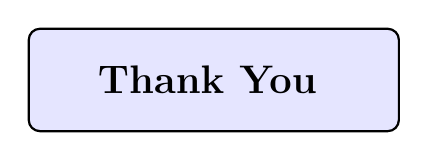
\begin{tikzpicture}
  \node[rectangle, rounded corners, draw, thick, fill=blue!10, minimum width=4.7cm, minimum height=1.3cm, align=center] {
    \Large \textbf{Thank You}
  };
\end{tikzpicture}

\vspace{0.8cm}

\end{frame}
\end{document}